\documentclass{article}
\usepackage{graphicx}
\usepackage{float}
\usepackage{booktabs}
\usepackage{hyperref}
\usepackage{rotating}

\usepackage{siunitx}
\usepackage{array}
\usepackage{amssymb}

\sisetup{
    table-number-alignment = center,
    round-mode = places,
    round-precision = 4
}

\usepackage[table]{xcolor}

\usepackage[a4paper,margin=1in]{geometry}

\title{DermFM-Zero-Open: Technical Report}
\author{Siyuan Yan, Xieji Li}
\date{September 2026}

\begin{document}

\maketitle

\section{Overview}
\label{sec:overview}

DermFM-Zero is a dermatology vision-language foundation model designed for zero-shot clinical decision support~\cite{dermfmzero}. This report introduces DermFM-Zero-Open, an openly releasable version trained exclusively on publicly available data. The original DermFM-Zero checkpoint cannot be released because its training corpus includes institutional data that are subject to data-sharing restrictions. Despite being trained only on public data, DermFM-Zero-Open achieves comparable performance to the original model across the same benchmarks, and outperforms it on several tasks.

DermFM-Zero-Open is initialized from the publicly released PanDerm vision encoder~\cite{panderm} and trained on 517,455 publicly sourced image-text pairs listed in Section~\ref{sec:data}. Training incorporates native-resolution inputs (Section~\ref{sec:navit}), multi-aspect knowledge contrastive learning (Section~\ref{sec:make}), and a knowledge-enhanced text encoder (Section~\ref{sec:kep}). Consequently, DermFM-Zero-Open differs from the checkpoint evaluated in the original paper in both its training corpus and training procedure. Results for the two checkpoints are reported side by side in Section~\ref{sec:benchmark} to characterize their relative performance, rather than as a strict reproduction of the published evaluation.

\section{Pretraining Data Statistics}
\label{sec:data}
\begin{table}[H]
    \centering
    \resizebox{0.7\linewidth}{!}{
    \begin{tabular}{l|lrr}
        \toprule
        Source & Captioning & Count & Percent (\%) \\
        \midrule
        Public (From DermNet) & MAGEN & 23882 & 4.6 \\
        IIYI & Derm1M & 53747 & 10.4 \\
        PubMed & Derm1M & 77552 & 15.0 \\
        Reddit & Derm1M & 1173 & 0.2 \\
        Textbook & Derm1M & 39656 & 7.7 \\
        Twitter & Derm1M & 6116 & 1.2 \\
        YouTube & Derm1M & 38297 & 7.4 \\
        Search-Engine & MAGEN & 150032 & 29.0 \\
        Dermweb & MAGEN & 26604 & 5.1 \\
        Derm12345 + Hiba & DermaSynth & 22961 & 4.4 \\
        ISIC & DermoGPT & 32651 & 6.3 \\
        MSKCC & MAGEN & 10618 & 2.1 \\
        BCN20000 & MAGEN & 17639 & 3.4 \\
        F17K & MAGEN & 16527 & 3.2 \\
        \midrule
        Total & -- & 517455 & 100.0 \\
        \bottomrule
    \end{tabular}
    }
\caption{Pretraining data sources of DermFM-Zero-Open.}
\label{tab:pretrain_data_statistics}
\end{table}

\begin{table}[H]
\centering
\resizebox{\textwidth}{!}{
\begin{tabular}{lccccccc}
\toprule
\textbf{Dataset}
& \textbf{HAM}
& \textbf{PAD}
& \textbf{ISIC2020}
& \textbf{PH2}
& \textbf{SNU}
& \textbf{SD-128}
& \textbf{Daffodil} \\
\midrule
Original size
& 1503
& 461
& 4969
& 200
& 2101
& 1405
& 1910 \\
Deduplicated size, original corpus
& 1488 (-15)
& 460 (-1)
& 4931 (-38)
& 175 (-25)
& 2098 (-3)
& 1383 (-22)
& 1651 (-259) \\
Overlap rate, original corpus
& 1.00\%
& 0.22\%
& 0.76\%
& 12.50\%
& 0.14\%
& 1.57\%
& 13.56\% \\
Overlap rate, retrained corpus
& 1.20\%
& 0.22\%
& 1.57\%
& 12.50\%
& 0.14\%
& 1.57\%
& 13.56\% \\
\bottomrule
\end{tabular}
}
\caption{Overlap between the pretraining corpora and the zero-shot benchmark datasets. Deduplicated sizes refer to the original corpus.}
\label{tab:pretrain_downstream_overlap}
\end{table}

\begin{figure}[H]
    \centering
    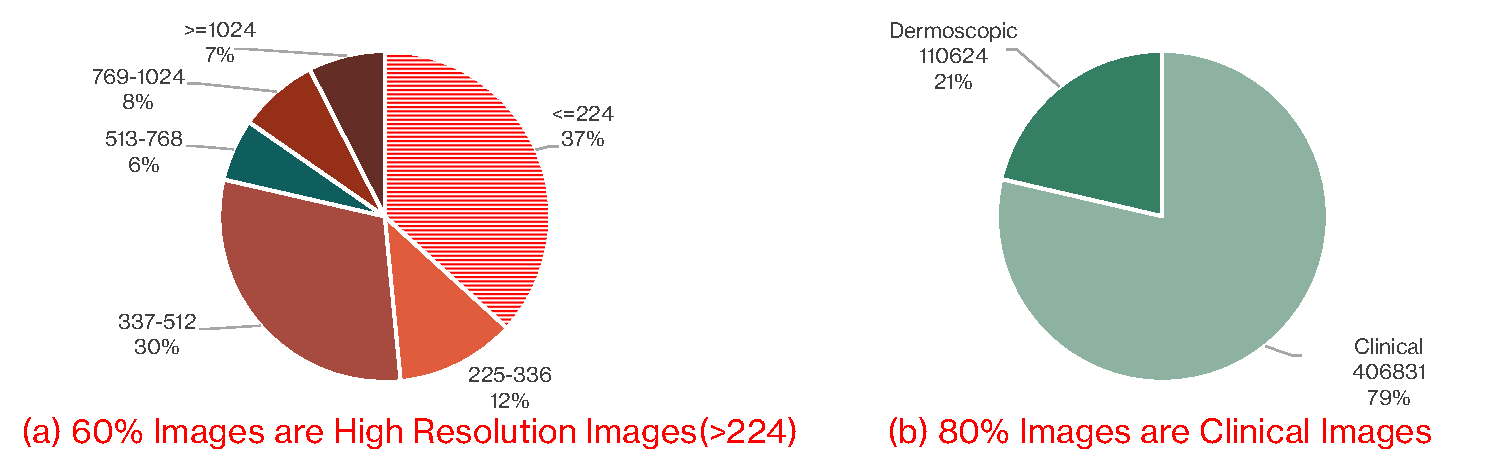
\includegraphics[width=\linewidth]{figures/pretrain-data-modalities-stats.pdf}
    \caption{Resolution and modality composition of the pretraining corpus. (a) More than 60\% of images exceed $224\times224$. (b) 406,831 images (79\%) are clinical photographs and 110,624 (21\%) are dermoscopic.}
    \label{fig:resolution-stats}
\end{figure}


\begin{figure}[H]
    \centering
    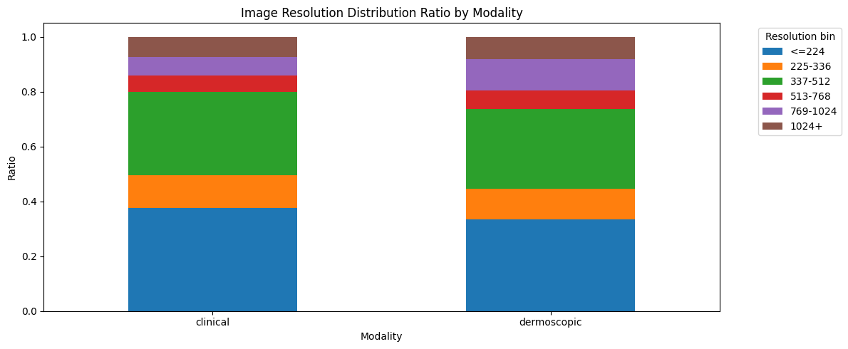
\includegraphics[width=0.8\linewidth]{figures/modality-stats.png}
    \caption{Resolution distributions are similar for clinical and dermoscopic images.}
    \label{fig:modality-resolution}
\end{figure}

\section{Method}

\subsection{Native Vision Input}
\label{sec:navit}

\paragraph{Motivation.}
Our previous vision backbone, PanDerm~\cite{panderm}, was pretrained by self-supervision on dermatology images at a fixed resolution of $224\times224$, the standard input size of vision transformers. This size does not match the resolution distribution of dermatology data: more than 60\% of the images in our pretraining corpus exceed $224\times224$ (Figure~\ref{fig:resolution-stats}a), and the two imaging modalities show the same pattern (Figure~\ref{fig:modality-resolution}). Downsampling these images to $224\times224$ removes fine-scale structure, including pigmentation patterns, vascular structures, and dermoscopic features such as the pigment network, dots, globules, and streaks. These are the features that separate benign from malignant lesions.

\paragraph{Patch-and-pack with a preserved PanDerm backbone.}
To accept native-resolution input while reusing PanDerm's pretrained weights, we adopt the patch-and-pack strategy of NaViT~\cite{dehghani2023patch}: patches from images of different sizes are packed into one sequence, and attention across images is masked (Figure~\ref{fig:navit}). The PanDerm backbone is unchanged; only the positional encoding is modified. PanDerm's absolute positional embeddings, defined on a $14\times14$ grid, are bilinearly interpolated to the patch grid of each input.

\paragraph{ScaleJitter.}
To make the representation less sensitive to input scale, we apply \emph{ScaleJitter} during pretraining: at each step, every image is resized to a randomly drawn scale within a fixed range, with its aspect ratio preserved. The encoder therefore sees the resolutions it will meet at inference, including web thumbnails, textbook scans, and native-resolution dermoscopy, and the resizing acts as an augmentation that complements patch-and-pack.

\paragraph{Implementation.}
We initialize the vision encoder from PanDerm and continue pretraining on the corpus of Section~\ref{sec:data}. ScaleJitter assigns each image one of three target short-side resolutions: the deployment resolution of $224$ with probability $0.5$; a value drawn uniformly from $[224,\, S_{\mathrm{native}}]$ with probability $0.25$, where $S_{\mathrm{native}}$ is the native short side; and the native resolution with the remaining probability $0.25$. The long side follows the aspect ratio up to a cap of $448$ pixels.

\begin{figure}[H]
    \centering
    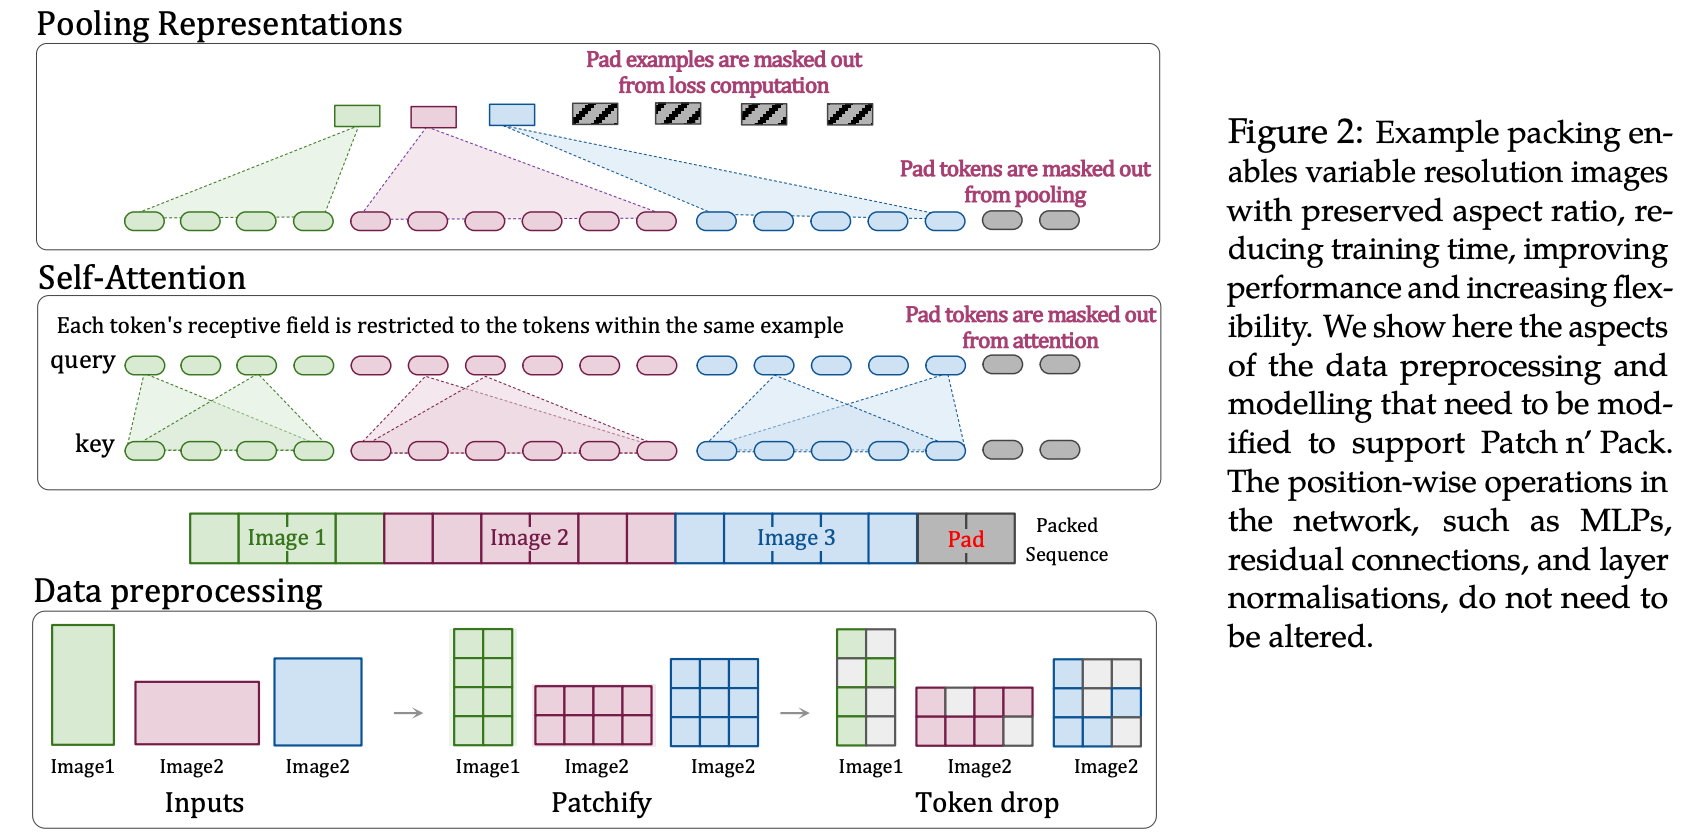
\includegraphics[width=1\linewidth]{figures/NaViT.png}
    \caption{The patch-and-pack strategy. Patches from images of different sizes are packed into one sequence, with attention across images masked.}
    \label{fig:navit}
\end{figure}

\subsection{Multi-Aspect Knowledge Contrastive Learning (MAKE)}
\label{sec:make}
\paragraph{Motivation.}
Standard CLIP-style pretraining aligns each image with a single caption truncated to the context length, so most of the clinical reasoning written alongside dermatology images is not used. Captions in our corpus describe a lesion from several angles: a diagnosis with its taxonomic ancestors, the morphological concepts a dermatologist would name on examination, and a multi-sentence narrative. We therefore adopt MAKE~\cite{make}, which aligns the image with all of these views at once through three components: multi-aspect contrastive learning, fine-grained alignment, and diagnosis-guided weighting (Figure~\ref{fig:make}). The MAKE baseline in Table~\ref{tab:zero_shot_benchmark} is the original model of that work; here we reuse its training objective inside our own encoder.

\paragraph{Multi-aspect text construction.}
For each image--text pair $(I_i, T_i^r)$, we build two sets of textual views. The \emph{knowledge set} $\{T_i^r,\, t_i^d,\, t_i^c\}$ combines the raw caption with two aspects extracted by a large language model: a disease aspect $t_i^d$ holding standardized diagnostic terms, synonyms, and taxonomic ancestors (e.g., melanoma $\rightarrow$ malignant), and a concept aspect $t_i^c$ listing the morphological descriptors named in the caption (e.g., plaque, scale, erosion). The \emph{subtext set} $S_i = \{S_i^j\}_{j=1}^{K}$ is obtained by splitting $T_i^r$ into sentences and keeps content that would otherwise be cut by the text encoder's context window. The vision encoder yields a global embedding $e_i^v = E_V(I_i)$ and patch embeddings $e_i^p = [v_i^1, \ldots, v_i^{HW}]$, and the text encoder produces $K{+}3$ embeddings per sample: $e_i^t = \bigl(e^r_i,\, e^d_i,\, e^c_i,\, \{e^{s_j}_i\}_{j=1}^K\bigr)$.

\paragraph{Multi-aspect contrastive learning.}
We align $e_i^v$ with all $K{+}3$ text embeddings using a symmetric
multi-positive contrastive loss. The image-to-text term is
\begin{equation}
\mathcal{L}_{i2t}^{mkcl} = -\sum_{i=1}^{N}\sum_{j \in \mathcal{J}}
\log \frac{\exp(\langle e_i^v, e_{ij}^t \rangle / \tau)}
         {\sum_{n=1}^{N}\exp(\langle e_n^v, e_{ij}^t \rangle / \tau)},
\end{equation}
where $\mathcal{J} = \{r, d, c, s_1, \ldots, s_K\}$ indexes the text
views and $\tau$ is a learnable temperature. The text-to-image term
$\mathcal{L}_{t2i}^{mkcl}$ is symmetric, and the overall objective is
$\mathcal{L}^{mkcl} = (\mathcal{L}_{i2t}^{mkcl} + \mathcal{L}_{t2i}^{mkcl})/2$.

\paragraph{Fine-grained alignment.}
Global image--text similarity does not capture where a described feature lies on the lesion. We therefore form a knowledge-enhanced visual embedding by pooling the patch tokens with weights given by their similarity to the raw caption:
\begin{equation}
z_i = e_i^r \cdot (e_i^p)^\top,
\qquad
e_i^k = \sum_{n=1}^{HW} v_i^n \cdot
        \frac{z_i^n}{\sum_{j=1}^{HW} z_i^j}.
\end{equation}
Each subtext is then aligned with $e_i^k$ rather than with the global $e_i^v$,
\begin{equation}
\mathcal{L}_{slra} = -\sum_{i=1}^{N}\sum_{j=1}^{K}
\log \frac{\exp(\langle e^{s_j}_i, e_i^k \rangle / \tau)}
         {\sum_{n=1}^{N} \exp(\langle e^{s_j}_i, e_n^k \rangle / \tau)},
\end{equation}
so that each sentence is matched to the patches most relevant to its content.

\paragraph{Diagnosis knowledge-guided weighting.}
Subtexts differ in diagnostic value: a sentence giving the patient's age carries less information than one describing lesion morphology. We therefore weight each subtext by its similarity to the disease aspect embedding $e_i^d$,
\begin{equation}
w_i^j = \frac{e_i^d \cdot (e_i^{s_j})^\top}
             {\max_{k}\, e_i^d \cdot (e_i^{s_k})^\top},
\qquad j = 1, \ldots, K.
\end{equation}
The knowledge-set embeddings ($e_i^r,\, e_i^d,\, e_i^c$) receive unit weight because they already hold condensed diagnostic information. In the released model this weighting is switched off, that is $w_i^j = 1$ for every subtext (Section~\ref{sec:implementation}).

\paragraph{Total objective.}
The MAKE loss combines the global and fine-grained terms under the diagnosis-guided weights,
\begin{equation}
\mathcal{L}_{\mathrm{MAKE}} = \lambda_m\, \hat{w}_{mkcl}\, \mathcal{L}^{mkcl}
                            + \lambda_s\, \hat{w}_{slra}\, \mathcal{L}_{slra},
\end{equation}
where $\hat{w}_{mkcl}$ and $\hat{w}_{slra}$ aggregate the per-subtext weights, and $\lambda_m$ and $\lambda_s$ balance the two terms. We set $\lambda_m = 1.0$ and $\lambda_s = 0.5$.

\begin{figure}[H]
    \centering
    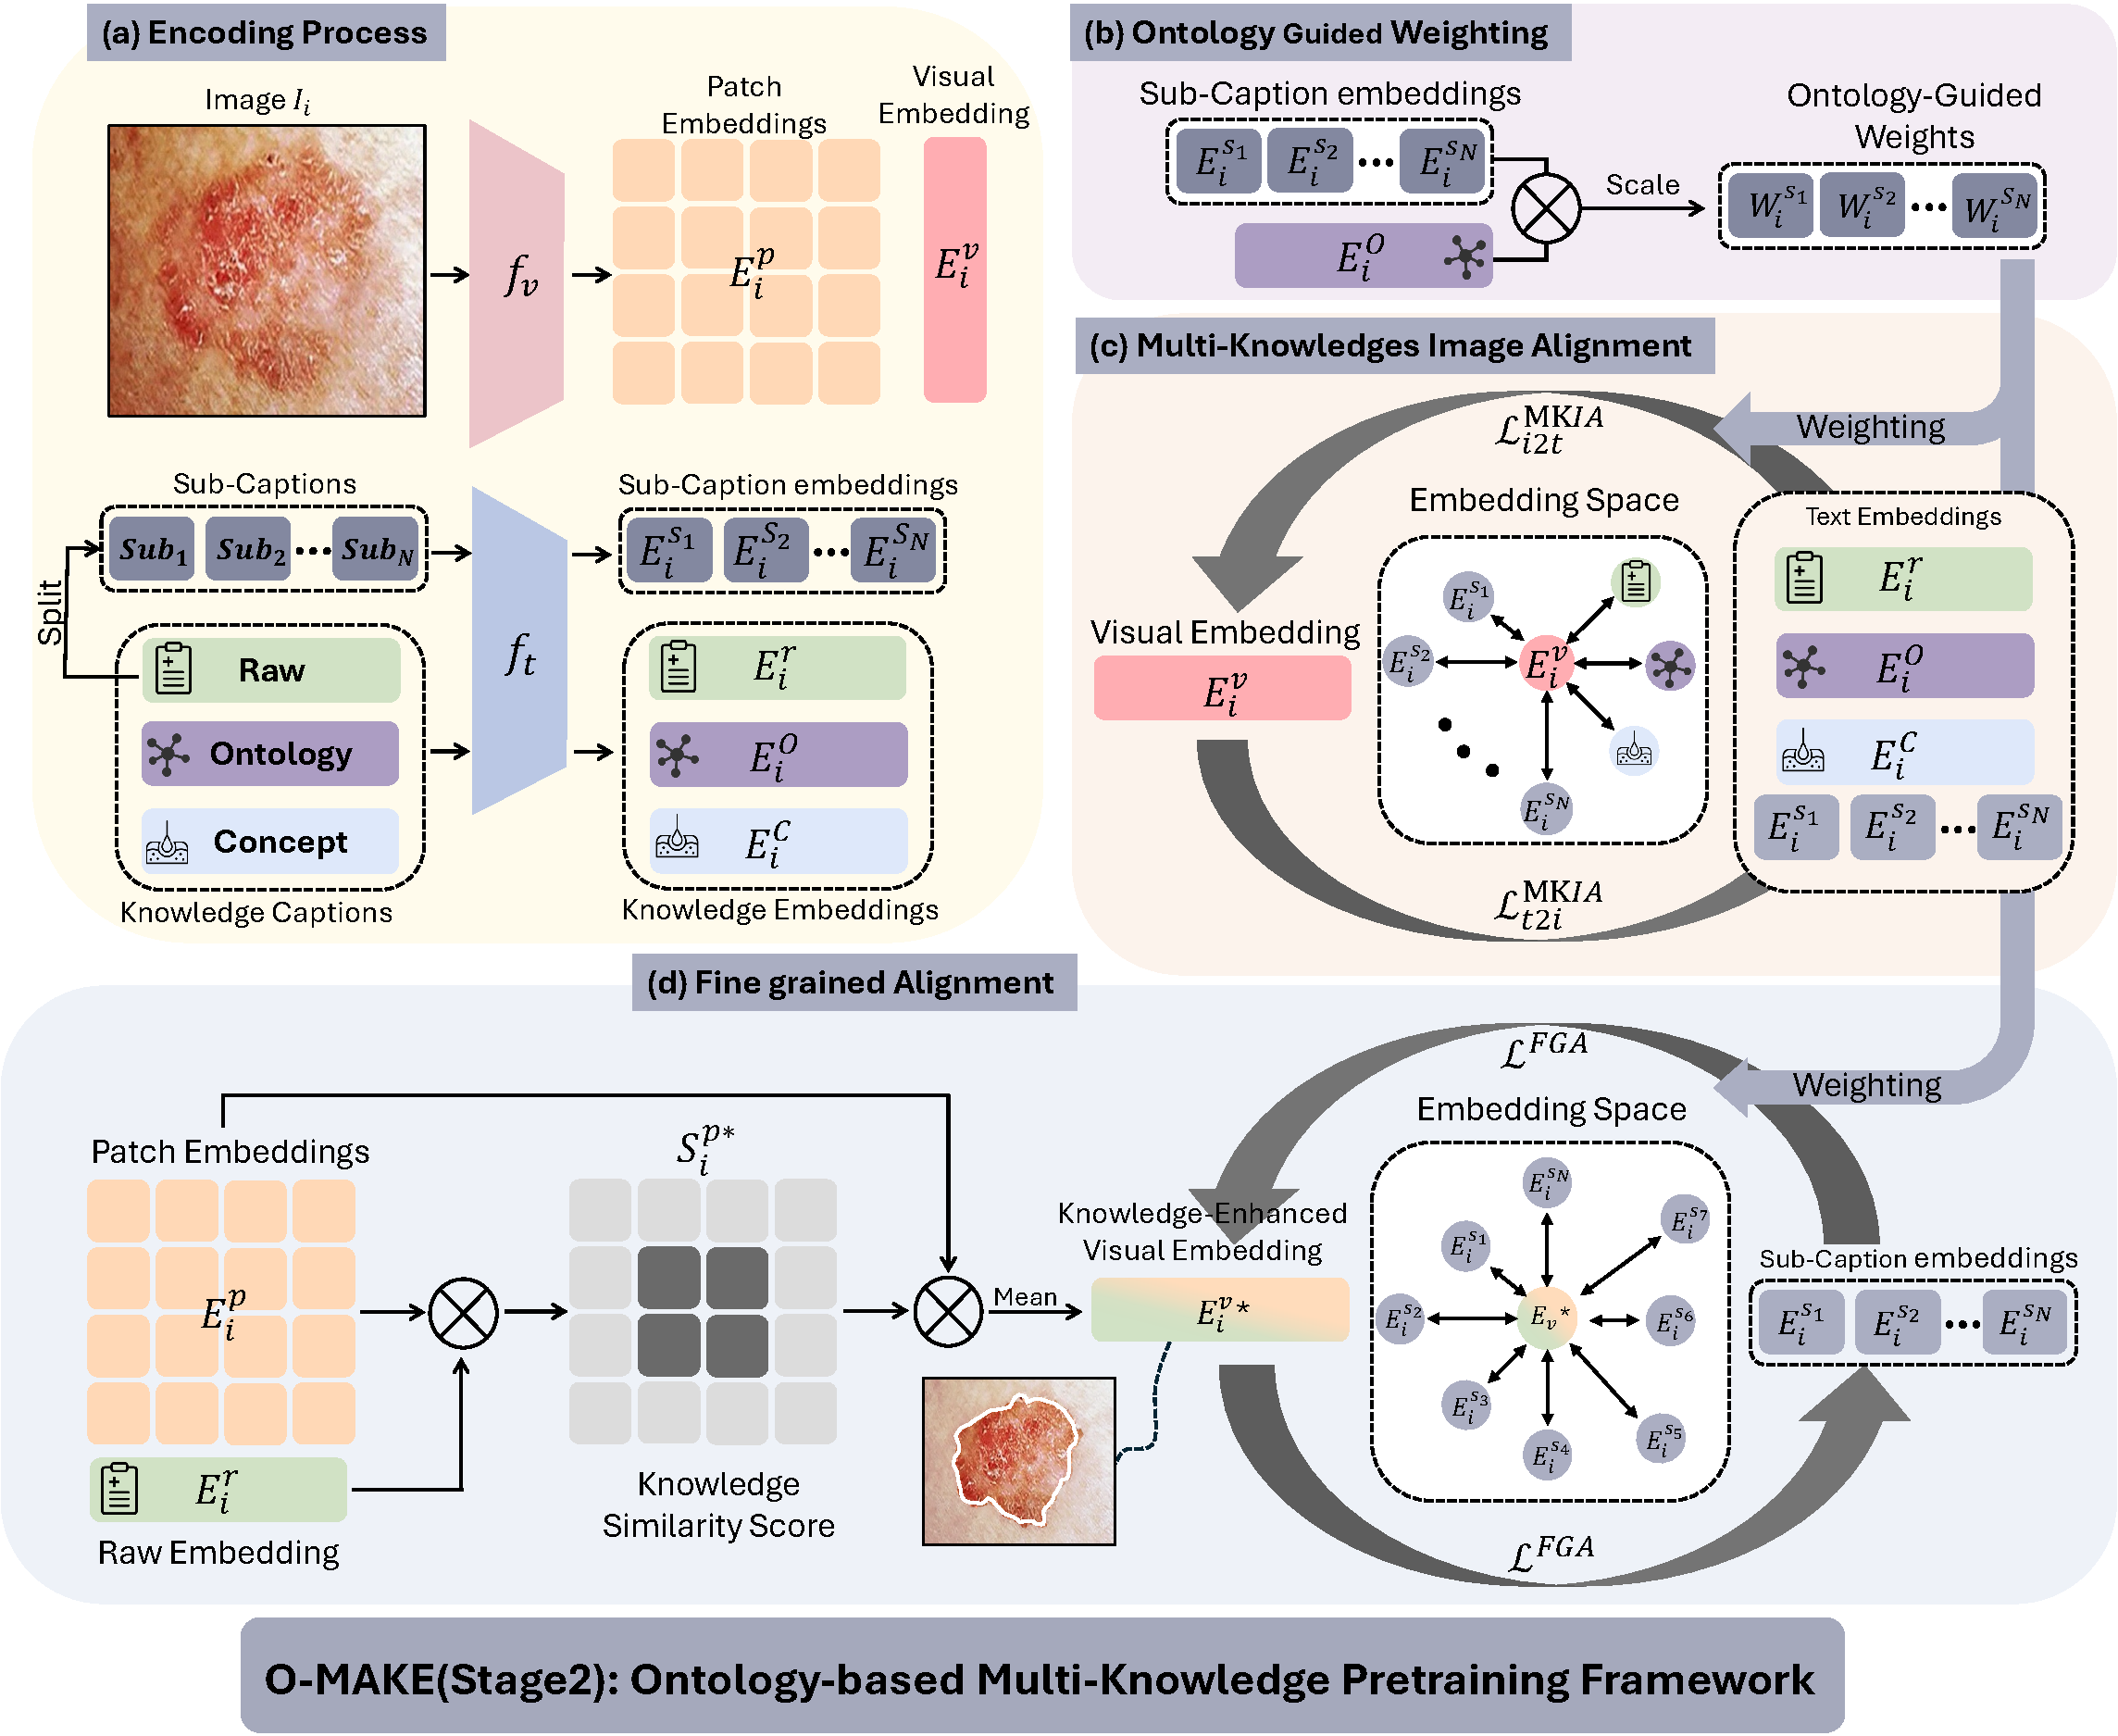
\includegraphics[width=0.7\linewidth]{figures/MAKE.pdf}
    \caption{Overview of multi-aspect knowledge contrastive learning (MAKE).}
    \label{fig:make}
\end{figure}

\subsection{Knowledge-Enhanced Text Encoder (KEP)}
\label{sec:kep}

\begin{figure}[H]
    \centering
    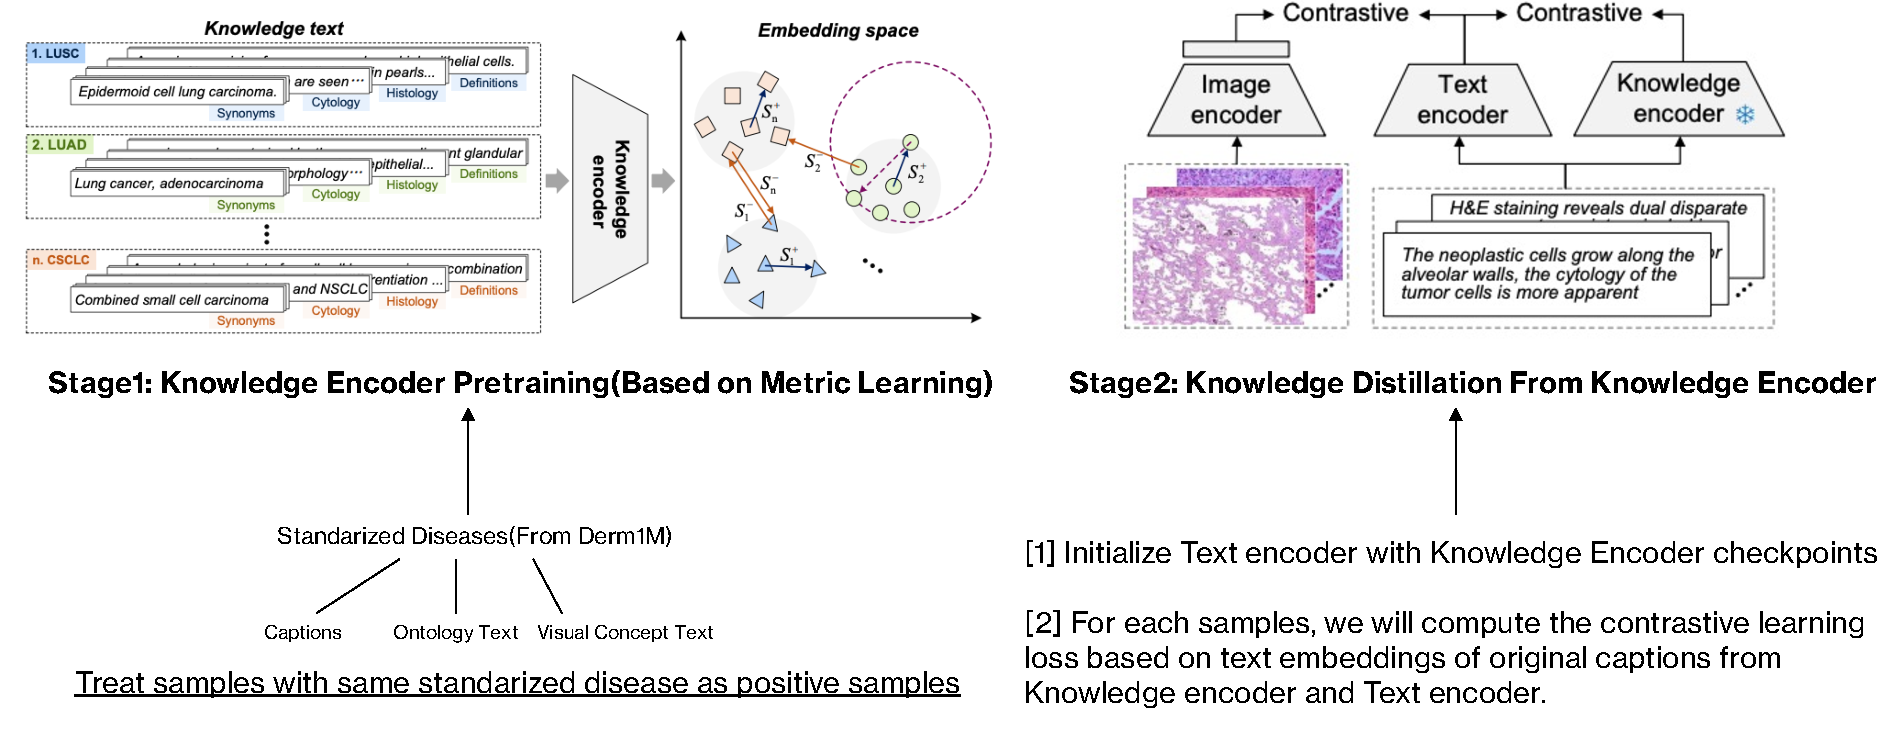
\includegraphics[width=1\linewidth]{figures/KEP.pdf}
    \caption{Knowledge-enhanced text encoder (KEP). The frozen knowledge encoder $E_K$ anchors the trainable CLIP text encoder $E_T$.}
    \label{fig:KEP}
\end{figure}

\paragraph{Motivation.}
The text encoder in CLIP-style pretraining is trained from scratch alongside the vision encoder and receives no supervision from structured medical knowledge. In dermatology this matters: one condition appears under several synonyms, sits in a defined taxonomic hierarchy, and is associated with a canonical set of visual concepts. Without this ontology, the text encoder may not recognize that ``naevus'' and ``nevus'' name the same entity, or that melanoma inherits the morphological vocabulary of pigmented lesions. To supply this prior, we adopt the two-stage Knowledge-Enhanced Pretraining (KEP) framework~\cite{KEP} and instantiate it for dermatology.

\paragraph{Text Encoder Pretraining: Dermatological knowledge tree and knowledge encoder.}
We replace KEP's pathology knowledge tree with a dermatological tree of skin-condition entities. Each entity is populated with attribute texts of six types, including raw captions, ontology captions (synonyms and taxonomic ancestors), visual concept captions (canonical morphological descriptors), and sub-captions obtained by splitting the raw text into sentences. The resulting corpus contains $556{,}372$ attribute texts. Following the original two-stage protocol with all hyperparameters unchanged, we train a PubMedBERT-based text encoder $E_K$ on this corpus with KEP's AdaSP loss, which pulls attribute texts of the same condition together and pushes apart those of different conditions. The resulting checkpoint outputs $768$-dimensional embeddings aligned with the dermatological ontology and serves as the frozen knowledge encoder in the image-text pretraining stage.

\paragraph{Image-Text Pretraining: Knowledge distillation contrastive learning.}

In the image-text pretraining stage, $E_K$ is frozen and anchors the trainable CLIP text encoder $E_T$ (Figure~\ref{fig:KEP}). For each image--text pair $(I_i, T_i^r)$, the raw caption is passed through both encoders, giving a knowledge embedding $e_i^{K} = E_K(T_i^r)$ and a CLIP text embedding $e_i^{r} = E_T(T_i^r)$. Because $E_K$ already outputs $768$-dimensional features matching the CLIP embedding space, no projection is inserted between the two streams. We apply a symmetric InfoNCE objective between them:
\begin{equation}
\label{eq:kd_loss}
\mathcal{L}_{\mathrm{KD}} = -\frac{1}{2N}\sum_{i=1}^{N}
\left[
\log \frac{\exp(\langle e_i^r, e_i^{K} \rangle / \tau)}
         {\sum_{n=1}^N \exp(\langle e_i^r, e_n^{K} \rangle / \tau)}
+
\log \frac{\exp(\langle e_i^{K}, e_i^r \rangle / \tau)}
         {\sum_{n=1}^N \exp(\langle e_i^{K}, e_n^r \rangle / \tau)}
\right],
\end{equation}
with the same temperature $\tau$ as the MAKE objective. This term pulls each CLIP text embedding toward its knowledge-encoder counterpart and away from those of other samples, so the ontology learned in the text encoder pretraining stage is distilled into $E_T$ without freezing or replacing it.

\paragraph{Total objective.}
The full DermFM-Zero-Open pretraining loss combines the MAKE objective (Section~\ref{sec:make}) with the KEP knowledge-distillation term,
\begin{equation}
\label{eq:total_loss}
\mathcal{L}_{\mathrm{total}} = \mathcal{L}_{\mathrm{MAKE}}
                             + \lambda_k\, \mathcal{L}_{\mathrm{KD}},
\end{equation}
where $\lambda_k$ sets the strength of the distillation signal; we use $\lambda_k = 0.4$.


\subsection{Pretraining Details}
\label{sec:implementation}
Our vision encoder is PanDerm-Large (ViT-L/16) extended with patch-and-pack. The trainable text encoder is the KEP PubMedBERT-256 tower, and the Stage-1 PubMedBERT-256 checkpoint serves as the frozen knowledge encoder; both produce $768$-dimensional embeddings, so no projection layer is needed between them. Each training sample provides one image and five caption views: the raw caption, the disease and concept aspects, and $K{=}2$ sub-captions obtained by sentence decomposition. Images are augmented with a random resized crop at scale $[0.4, 1.0]$, color jitter with parameters $(0.32, 0.32, 0.32, 0.08)$ applied with probability $0.8$, and grayscale conversion with probability $0.2$. ScaleJitter then sets the short side as described in Section~\ref{sec:navit}. We optimize with AdamW ($\beta_1{=}0.9$, $\beta_2{=}0.98$, weight decay $0.1$); the learning rate is warmed up to $1\!\times\!10^{-4}$ over $200$ steps and then decays to zero on a cosine schedule. Training runs for $15$ epochs on two GPUs with a per-device batch size of $512$ and gradient accumulation factor $2$, an effective batch size of $2{,}048$, using bf16 mixed precision, gradient checkpointing in the vision tower, gradient clipping at norm $5.0$, and the local-loss variant of \texttt{open\_clip}. The three loss components are weighted as $\lambda_m{=}1.0$, $\lambda_s{=}0.5$, and $\lambda_k{=}0.4$, with diagnosis knowledge-guided weighting disabled.

\section{Benchmark}
\label{sec:benchmark}

We evaluate DermFM-Zero-Open under the protocols of the main paper: zero-shot classification, linear probing, zero-shot retrieval, multimodal finetuning, visual question answering, and automated concept discovery. \emph{Zero-shot classification} tests the alignment between the vision and text encoders without task-specific training, and \emph{linear probing} measures the linear separability of the frozen visual features under full supervision. In every table, DermFM-Zero denotes the checkpoint evaluated in the paper and DermFM-Zero-Open the released checkpoint retrained on the corpus of Section~\ref{sec:data}.

\paragraph{Fair-comparison setup.}
Native-resolution pretraining yields an encoder that accepts inputs of any size, whereas several baselines operate at a fixed $224\times224$ input. For a like-for-like comparison, we evaluate DermFM-Zero-Open at $224\times224$ on all benchmarks. Section~\ref{sec:ablation} compares the two inference resolutions for the MAKE + NaViT configuration.

\paragraph{Zero-shot classification.}
DermFM-Zero-Open averages 0.6909 across the seven benchmarks, ahead of the strongest open baseline, DermLIP, at 0.5640 and of the best general-purpose model, GPT-4o, at 0.5106 (Table~\ref{tab:zero_shot_benchmark}). It also exceeds the paper checkpoint, which averages 0.6750 under the same metrics, and leads on PAD, ISIC2020, PH2 and SD-128; the paper checkpoint stays ahead on HAM, SNU and DAFFODIL.

\begin{table}[H]
\centering
\caption{Zero-shot classification on seven dermatology benchmarks. Top-1 accuracy is reported for the five multi-class datasets and macro F1 for the two binary datasets (ISIC2020, PH2). The benchmark table in the code repository reports AUROC for these two datasets, so the averages in the two documents are not directly comparable. DermFM-Zero-Open is evaluated at $224\times224$. Best value per column in bold.}
\label{tab:zero_shot_benchmark}
\resizebox{\textwidth}{!}{
\begin{tabular}{
    l
    S[table-format=1.4]
    S[table-format=1.4]
    S[table-format=1.4]
    S[table-format=1.4]
    S[table-format=1.4]
    S[table-format=1.4]
    S[table-format=1.4]
    S[table-format=1.4]
}
\toprule
\textbf{Model} 
& {\textbf{HAM}} 
& {\textbf{PAD}} 
& {\textbf{ISIC2020}} 
& {\textbf{PH2}} 
& {\textbf{SNU}} 
& {\textbf{SD-128}} 
& {\textbf{Daffodil}} 
& {\textbf{Average}} \\
\midrule
Task 
& {Skin Cancer} 
& {Skin Cancer} 
& {Mel Det.} 
& {Mel Det.} 
& {DDX} 
& {DDX} 
& {Rare DX} 
& {--} \\
Size 
& {1503} 
& {461} 
& {4969} 
& {200} 
& {2101} 
& {1405} 
& {1910} 
& {--} \\
Class-modal 
& {7-D} 
& {6-C} 
& {2-D} 
& {2-D} 
& {134-C} 
& {128-C} 
& {5-D} 
& {--} \\
Country/Inst. 
& {Austria} 
& {Brazil} 
& {Multi-center} 
& {Portugal} 
& {Korea} 
& {Multi-center} 
& {Multi-center} 
& {--} \\
Metric 
& {ACC} 
& {ACC} 
& {Macro F1} 
& {Macro F1} 
& {ACC} 
& {ACC} 
& {ACC} 
& {--} \\
\midrule
CLIP-L/14 & 0.2754 & 0.3839 & 0.4896 & 0.4494 & 0.0857 & 0.1210 & 0.5304 & 0.3336 \\
BiomedCLIP & 0.6347 & 0.4512 & 0.5317 & 0.6292 & 0.0966 & 0.1153 & 0.5785 & 0.4339 \\
MMKD-CLIP & 0.3174 & 0.3471 & 0.4884 & 0.6988 & 0.1052 & 0.0961 & 0.5586 & 0.3731 \\
MedSigLIP & 0.4604 & 0.6464 & 0.5409 & 0.7938 & 0.2213 & 0.2028 & 0.6089 & 0.4964 \\
BMC-CLIP & 0.4717 & 0.5206 & 0.5257 & 0.4867 & 0.1395 & 0.1345 & 0.6974 & 0.4252 \\
DermLIP & 0.6281 & 0.6247 & 0.5190 & 0.6799 & 0.3332 & 0.3822 & 0.7812 & 0.5640 \\
MONET & 0.3347 & 0.4729 & 0.5208 & 0.6774 & 0.1414 & 0.2028 & 0.7607 & 0.4444 \\
MAKE & 0.4551 & 0.5857 & 0.4259 & 0.8222 & 0.3260 & 0.3886 & 0.7785 & 0.5403 \\
\midrule
GPT-4o & 0.3766 & 0.5748 & 0.5329 & 0.7010 & 0.2734 & 0.3174 & 0.7948 & 0.5106 \\
Gemini-2.5-pro (Think) & 0.3094 & 0.5965 & 0.3760 & 0.5236 & 0.2851 & 0.4064 & 0.8450 & 0.4775 \\
GPT-5.2-pro & 0.3147 & 0.6052 & 0.4972 & 0.6842 & 0.2109 & 0.3402 & 0.7283 & 0.4830 \\
\midrule
\rowcolor{gray!25}
\textbf{DermFM-Zero} 
& {\textbf{0.7957}} 
& 0.6941 
& 0.5979 
& 0.7998 
& {\textbf{0.4450}} 
& 0.5075 
& {\textbf{0.8848}} 
& 0.6750 \\
\rowcolor{gray!25}
\textbf{DermFM-Zero-Open} 
& 0.7858 
& {\textbf{0.7592}} 
& {\textbf{0.6112}} 
& {\textbf{0.8708}} 
& 0.4212 
& {\textbf{0.5196}} 
& 0.8686 
& {\textbf{0.6909}} \\
\bottomrule
\end{tabular}
}
\end{table}

\subsection{Linear Probing}

DermFM-Zero-Open gives the higher average at every label fraction: 0.7490 at 10\%, 0.7976 at 30\%, 0.8123 at 50\% and 0.8313 at 100\% (Tables~\ref{tab:lp_10_benchmark}--\ref{tab:lp_100_benchmark}). The margin over the paper checkpoint is largest with the fewest labels, 0.050 at 10\%, and falls to 0.006 at 100\%, so most of the benefit of the retrained encoder appears in the low-label regime.

\begin{table}[H]
\centering
\resizebox{0.75\textwidth}{!}{
\begin{tabular}{
    l
    S[table-format=1.4]
    S[table-format=1.4]
    S[table-format=1.4]
    S[table-format=1.4]
    S[table-format=1.4]
}
\toprule
\textbf{Model}
& {\textbf{HAM}}
& {\textbf{ISIC2020}}
& {\textbf{PAD}}
& {\textbf{SD-128}}
& {\textbf{Average}} \\
\midrule
Task
& {Skin Cancer}
& {Mel Det.}
& {Skin Cancer}
& {DDX}
& {--} \\
Size
& {1503}
& {4969}
& {461}
& {1405}
& {--} \\
Class-modal
& {7-D}
& {2-D}
& {6-C}
& {128-C}
& {--} \\
Metric
& {top1 ACC}
& {AUROC}
& {top1 ACC}
& {top1 ACC}
& {--} \\
\midrule
Derm-foundation & 0.7725 & 0.7942 & 0.6789 & 0.3708 & 0.6541 \\
MMKD-CLIP       & 0.7445 & 0.7615 & 0.5662 & 0.2085 & 0.5702 \\
MedSigLIP       & 0.7997 & 0.8033 & 0.6790 & 0.3587 & 0.6602 \\
BMC-CLIP        & 0.7951 & 0.8144 & 0.6594 & 0.3181 & 0.6468 \\
\midrule
\rowcolor{gray!15}
\textbf{DermFM-Zero}
& 0.8416
& 0.8687
& 0.6855
& 0.4007
& 0.6991 \\
\rowcolor{gray!15}
\textbf{DermFM-Zero-Open}
& {\textbf{0.8629}}
& {\textbf{0.9008}}
& {\textbf{0.7527}}
& {\textbf{0.4797}}
& {\textbf{0.7490}} \\
\bottomrule
\end{tabular}
}
\caption{Linear probing with 10\% of the training data. The best value in each column is in bold.}
\label{tab:lp_10_benchmark}
\end{table}

\begin{table}[H]
\centering
\resizebox{0.75\textwidth}{!}{
\begin{tabular}{
    l
    S[table-format=1.4]
    S[table-format=1.4]
    S[table-format=1.4]
    S[table-format=1.4]
    S[table-format=1.4]
}
\toprule
\textbf{Model}
& {\textbf{HAM}}
& {\textbf{ISIC2020}}
& {\textbf{PAD}}
& {\textbf{SD-128}}
& {\textbf{Average}} \\
\midrule
Task
& {Skin Cancer}
& {Mel Det.}
& {Skin Cancer}
& {DDX}
& {--} \\
Size
& {1503}
& {4969}
& {461}
& {1405}
& {--} \\
Class-modal
& {7-D}
& {2-D}
& {6-C}
& {128-C}
& {--} \\
Metric
& {top1 ACC}
& {AUROC}
& {top1 ACC}
& {top1 ACC}
& {--} \\
\midrule
Derm-foundation & 0.8224 & 0.8563 & \textbf{0.7809} & 0.5345 & 0.7485 \\
MMKD-CLIP       & 0.7598 & 0.8217 & 0.6182 & 0.3089 & 0.6271 \\
MedSigLIP       & 0.8423 & 0.8417 & 0.7050 & 0.5523 & 0.7353 \\
BMC-CLIP        & 0.8277 & 0.8527 & 0.7050 & 0.4911 & 0.7191 \\
\midrule
\rowcolor{gray!15}
\textbf{DermFM-Zero}
& {0.8769}
& \textbf{0.9239}
& 0.7223
& 0.5851
& 0.7771 \\
\rowcolor{gray!15}
\textbf{DermFM-Zero-Open}
& \textbf{0.8876}
& {0.9150}
& 0.7636
& {\textbf{0.6242}}
& {\textbf{0.7976}} \\
\bottomrule
\end{tabular}
}
\caption{Linear probing with 30\% of the training data. The best value in each column is in bold.}
\label{tab:lp_30_benchmark}
\end{table}

\begin{table}[H]
\centering

\resizebox{0.75\textwidth}{!}{
\begin{tabular}{
    l
    S[table-format=1.4]
    S[table-format=1.4]
    S[table-format=1.4]
    S[table-format=1.4]
    S[table-format=1.4]
}
\toprule
\textbf{Model}
& {\textbf{HAM}}
& {\textbf{ISIC2020}}
& {\textbf{PAD}}
& {\textbf{SD-128}}
& {\textbf{Average}} \\
\midrule
Task
& {Skin Cancer}
& {Mel Det.}
& {Skin Cancer}
& {DDX}
& {--} \\
Size
& {1503}
& {4969}
& {461}
& {1405}
& {--} \\
Class-modal
& {7-D}
& {2-D}
& {6-C}
& {128-C}
& {--} \\
Metric
& {top1 ACC}
& {AUROC}
& {top1 ACC}
& {top1 ACC}
& {--} \\
\midrule
Derm-foundation & 0.8323 & 0.8467 & 0.7722 & 0.5986 & 0.7625 \\
MMKD-CLIP       & 0.7784 & 0.8320 & 0.5944 & 0.3488 & 0.6384 \\
MedSigLIP       & 0.8683 & 0.8469 & 0.7202 & 0.6057 & 0.7603 \\
BMC-CLIP        & 0.8417 & 0.8658 & 0.7072 & 0.5359 & 0.7377 \\
\midrule
\rowcolor{gray!15}
\textbf{DermFM-Zero}
& {\textbf{0.8916}}
& {\textbf{0.9348}}
& 0.7505
& 0.6534
& 0.8076 \\
\rowcolor{gray!15}
\textbf{DermFM-Zero-Open}
& 0.8869
& 0.9174
& {\textbf{0.7852}}
& \textbf{0.6598}
& {\textbf{0.8123}} \\
\bottomrule
\end{tabular}
}
\caption{Linear probing with 50\% of the training data. The best value in each column is in bold.}
\label{tab:lp_50_benchmark}
\end{table}

\begin{table}[H]
\centering
\resizebox{0.75\textwidth}{!}{
\begin{tabular}{
    l
    S[table-format=1.4]
    S[table-format=1.4]
    S[table-format=1.4]
    S[table-format=1.4]
    S[table-format=1.4]
}
\toprule
\textbf{Model}
& {\textbf{HAM}}
& {\textbf{ISIC2020}}
& {\textbf{PAD}}
& {\textbf{SD-128}}
& {\textbf{Average}} \\
\midrule
Task
& {Skin Cancer}
& {Mel Det.}
& {Skin Cancer}
& {DDX}
& {--} \\
Size
& {1503}
& {4969}
& {461}
& {1405}
& {--} \\
Class-modal
& {7-D}
& {2-D}
& {6-C}
& {128-C}
& {--} \\
Metric
& {top1 ACC}
& {AUROC}
& {top1 ACC}
& {top1 ACC}
& {--} \\
\midrule
Derm-foundation & 0.8510 & 0.9077 & 0.7636 & 0.6854 & 0.8019 \\
MMKD-CLIP       & 0.7858 & 0.8287 & 0.6855 & 0.3964 & 0.6741 \\
MedSigLIP       & 0.8769 & 0.8465 & 0.7701 & 0.6840 & 0.7944 \\
BMC-CLIP        & 0.8649 & 0.8738 & 0.7397 & 0.6263 & 0.7762 \\
\midrule
\rowcolor{gray!15}
\textbf{DermFM-Zero}
& {0.8929}
& {\textbf{0.9386}}
& 0.7549
& {\textbf{0.7139}}
& 0.8251 \\
\rowcolor{gray!15}
\textbf{DermFM-Zero-Open}
& \textbf{0.8955}
& 0.9181
& {\textbf{0.8026}}
& 0.7032
& {\textbf{0.8313}} \\
\bottomrule
\end{tabular}
}
\caption{Linear probing with 100\% of the training data. The best value in each column is in bold.}
\label{tab:lp_100_benchmark}
\end{table}

\subsection{Zero-shot Retrieval}

The two retrieval sets separate the checkpoints. On SkinCap, DermFM-Zero-Open retrieves better at every cut-off in both directions, with I2T R@5 of 0.2231 against 0.1930 (Table~\ref{tab:retrieval_benchmark}). On the Derm1M hold-out set the order reverses, with I2T R@5 of 0.2522 against 0.3574 (Table~\ref{tab:derm1m_holdout_retrieval}). The retrained corpus holds 517,455 image-text pairs against 1,014,085 for the paper checkpoint, and the hold-out pairs are excluded from both.

\begin{table}[H]
\centering
\resizebox{0.75\textwidth}{!}{
\begin{tabular}{
    l
    S[table-format=1.4]
    S[table-format=1.4]
    S[table-format=1.4]
    S[table-format=1.4]
    S[table-format=1.4]
    S[table-format=1.4]
}
\toprule
\textbf{Method}
& \multicolumn{3}{c}{\textbf{I2T}}
& \multicolumn{3}{c}{\textbf{T2I}} \\
\cmidrule(lr){2-4} \cmidrule(lr){5-7}
& {R@5} & {R@10} & {R@50}
& {R@5} & {R@10} & {R@50} \\
\midrule
CLIP        & 0.0797 & 0.1289 & 0.3181 & 0.0569 & 0.0920 & 0.2344 \\
BiomedCLIP  & 0.0840 & 0.1356 & 0.3434 & 0.0750 & 0.1228 & 0.3294 \\
MONET       & 0.1048 & 0.1645 & 0.3863 & 0.0983 & 0.1574 & 0.3597 \\
DermFM-Zero   & {0.1930} & {0.3068} & {0.6257} & 0.1833 & 0.2885 & 0.5886 \\
\midrule
\rowcolor{gray!15}
\textbf{DermFM-Zero-Open}
& \textbf{0.2231} & \textbf{0.3447} & \textbf{0.6317} & \textbf{0.1990} & \textbf{0.3141} & \textbf{0.6337} \\
\bottomrule
\end{tabular}
}
\caption{Image-to-text (I2T) and text-to-image (T2I) retrieval on SkinCap (Recall@K).}
\label{tab:retrieval_benchmark}
\end{table}

\begin{table}[H]
\centering
\resizebox{0.75\textwidth}{!}{
\begin{tabular}{
    l
    S[table-format=1.4]
    S[table-format=1.4]
    S[table-format=1.4]
    S[table-format=1.4]
    S[table-format=1.4]
    S[table-format=1.4]
}
\toprule
\textbf{Method}
& \multicolumn{3}{c}{\textbf{I2T}}
& \multicolumn{3}{c}{\textbf{T2I}} \\
\cmidrule(lr){2-4} \cmidrule(lr){5-7}
& {R@5} & {R@10} & {R@50}
& {R@5} & {R@10} & {R@50} \\
\midrule
CLIP            & 0.0705 & 0.1001 & 0.2006 & 0.0552 & 0.0798 & 0.1790 \\
BiomedCLIP      & 0.1273 & 0.1659 & 0.2787 & 0.1139 & 0.1540 & 0.2757 \\
MONET           & 0.1043 & 0.1449 & 0.2709 & 0.0934 & 0.1283 & 0.2604 \\
DermFM-Zero & \textbf{0.3574} & \textbf{0.4341} & \textbf{0.6023} & \textbf{0.3517} & \textbf{0.4316} & \textbf{0.5980} \\
\midrule
\rowcolor{gray!15}
\textbf{DermFM-Zero-Open}
& 0.2522 & 0.3282 & 0.5131 & 0.2540 & 0.3332 & 0.5144 \\
\bottomrule
\end{tabular}
}
\caption{Image-to-text (I2T) and text-to-image (T2I) retrieval on the Derm1M hold-out set (Recall@K).}
\label{tab:derm1m_holdout_retrieval}
\end{table}

\subsection{Multimodal Finetuning}

Fine-tuned on the clinical, dermoscopic and metadata streams of Derm7pt, DermFM-Zero-Open reaches an F1 of 0.7710 against 0.7477 for the paper checkpoint and 0.6276 for the strongest non-dermatology backbone, CLIP-L/14 (Table~\ref{tab:derm7pt_multimodal_ft}).

\begin{table}[H]
\centering
\resizebox{0.45\textwidth}{!}{
\begin{tabular}{
    l
    S[table-format=1.4]
}
\toprule
\textbf{Backbone}
& {\textbf{Derm7Pt}} \\
\midrule
Metric
& {F1} \\
Classes
& {5} \\
Size (cases)
& {1011} \\
\midrule
CLIP-L14            & 0.6276 \\
BiomedCLIP          & 0.4595 \\
MONET               & 0.5366 \\
PanDerm-MLP         & 0.5418 \\
PanDerm-GPT77       & 0.5908 \\
DermFM-Zero     & 0.7477 \\
\midrule
\rowcolor{gray!15}
\textbf{DermFM-Zero-Open}
& {\textbf{0.7710}} \\
\bottomrule
\end{tabular}
}
\caption{Multimodal finetuning on Derm7pt (F1 score).}
\label{tab:derm7pt_multimodal_ft}
\end{table}

\subsection{VQA}

On Derm7pt-VQA, DermFM-Zero-Open gives the higher accuracy, 0.5441 against 0.5365, and the lower F1, 0.3373 against 0.3661 (Table~\ref{tab:vqa_benchmark}). On SkinCap-VQA the two checkpoints match on accuracy at 0.3702, with F1 of 0.1852 against 0.1949. Both remain above every baseline on accuracy.

\begin{table}[H]
\centering
\resizebox{0.7\textwidth}{!}{
\begin{tabular}{
    l
    c
    c
}
\toprule
\textbf{Backbone}
& {\textbf{Derm7pt-VQA}}
& {\textbf{SkinCap-VQA}} \\
\midrule
Metric
& {ACC/F1}
& {ACC/F1} \\
Answer Num
& {49}
& {188} \\
\midrule
BiomedCLIP      & 0.4912/0.2560 & 0.2858/0.0901 \\
CLIP-L14        & 0.5214/0.3153 & 0.2859/0.1242 \\
MONET           & 0.5290/0.3146 & 0.2859/0.1054 \\
DermFM-Zero & 0.5365/\textbf{0.3661} & \textbf{0.3702/0.1949} \\
\midrule
\rowcolor{gray!15}
\textbf{DermFM-Zero-Open}
& \textbf{0.5441}/0.3373
& 0.3702/0.1852 \\
\bottomrule
\end{tabular}
}
\caption{Visual question answering on Derm7pt-VQA (49 answers) and SkinCap-VQA (188 answers), reported as accuracy/F1.}
\label{tab:vqa_benchmark}
\end{table}

\subsection{Automated Concept Discovery}

Concepts discovered without supervision support both diagnostic tasks, with AUROC of 0.938 on clinical malignancy and 0.927 on dermoscopic melanoma (Table~\ref{tab:acd_cbm}). Suppressing the concepts that encode imaging artifacts restores accuracy on the three biased ISIC subsets, with the largest recovery on pen ink, from 0.057 to 0.617 (Table~\ref{tab:concept_intervention}).

\begin{table}[H]
\centering
\resizebox{0.55\textwidth}{!}{
\begin{tabular}{
    l
    S[table-format=1.3]
    S[table-format=1.3]
}
\toprule
\textbf{Classification Task}
& {\textbf{SAE-CBM}}
& {\textbf{Linear probe}} \\
\midrule
Clinical malignancy (F17K + DDI, $n=3{,}056$)   & 0.938 & 0.957 \\
Dermoscopic melanoma (Derm7pt, $n=827$)         & 0.927 & 0.932 \\
\bottomrule
\end{tabular}
}
\caption{Automated concept discovery (AUROC). SAE-CBM is a concept bottleneck model trained on the concepts discovered by the sparse autoencoder, averaged over 50 runs; Linear probe is the black-box upper bound on the same features.}
\label{tab:acd_cbm}
\end{table}

\begin{table}[H]
\centering
\resizebox{0.7\textwidth}{!}{
\begin{tabular}{
    l
    S[table-format=1.3]
    S[table-format=1.3]
    S[table-format=+1.3]
}
\toprule
\textbf{Concept Intervention (Debiasing)}
& {\textbf{Before}}
& {\textbf{After}}
& {\textbf{$(+)\Delta$}} \\
\midrule
ISIC $\cdot$ hair bias   & 0.637 & 0.868 & +0.231 \\
ISIC $\cdot$ ink bias    & 0.057 & 0.617 & +0.560 \\
ISIC $\cdot$ ruler bias  & 0.589 & 0.733 & +0.144 \\
\bottomrule
\end{tabular}
}
\caption{Concept intervention. AUROC before and after suppressing the artifact-related concepts in three biased ISIC subsets.}
\label{tab:concept_intervention}
\end{table}


\section{Ablation Study}
\label{sec:ablation}

Adding KEP to MAKE raises the zero-shot average from 0.6737 to 0.6832, and adding NaViT on top of both gives 0.6909, the released configuration (Table~\ref{tab:module_ablation_zero_shot}). For MAKE + NaViT, native-resolution inference scores 0.6539 against 0.6331 at $224\times224$; the gap comes almost entirely from PH2, where the two resolutions give 0.6898 and 0.4825 on 200 images.

\begin{table}[H]
\centering
\resizebox{\textwidth}{!}{
\begin{tabular}{ccc|cccccccc}
\toprule
\multicolumn{3}{c|}{\textbf{Zero-Shot Benchmark}}
& \textbf{Skin Cancer}
& \textbf{Skin Cancer}
& \textbf{Mel Det.}
& \textbf{Mel Det.}
& \textbf{DDX}
& \textbf{DDX}
& \textbf{Rare DX}
& \textbf{Average} \\
\midrule
\multicolumn{3}{c|}{Size}
& 1503 & 461 & 4969 & 200 & 2101 & 1405 & 1910 & -- \\
\multicolumn{3}{c|}{Dataset}
& HAM & PAD & ISIC2020 & PH2 & SNU & SD-128 & Daffodil & -- \\
\multicolumn{3}{c|}{Class-modal}
& 7-D & 6-C & 2-D & 2-D & 134-C & 128-C & 5-D & -- \\
\multicolumn{3}{c|}{Country/Inst.}
& Austria & Brazil & Multi-center & Portugal & Korea & Multi-center & Multi-center & -- \\
\multicolumn{3}{c|}{Metric}
& top1 ACC & top1 ACC & Macro F1 & Macro F1 & top1 ACC & top1 ACC & top1 ACC & -- \\
\midrule
\rowcolor{gray!15}
\multicolumn{3}{c|}{\textbf{DermFM-Zero}}
& \textbf{0.7957} & 0.6941 & 0.5979 & 0.7998 & \textbf{0.4450} & 0.5075 & \textbf{0.8848} & 0.6750 \\
\midrule
\textbf{MAKE}
& \textbf{KEP}
& \textbf{NaViT}
& \multicolumn{8}{c}{\textbf{Module Ablation}} \\
\midrule
$\checkmark$ & &
& 0.7804 & 0.6790 & 0.6158 & 0.8506 & 0.4265 & 0.4904 & 0.8733 & 0.6737 \\
$\checkmark$ & $\checkmark$ &
& 0.7944 & 0.7007 & 0.6261 & 0.8605 & 0.4150 & 0.5032 & 0.8822 & 0.6832 \\
$\checkmark$ & & $\checkmark^{*}$
& 0.8077 & 0.7093 & \textbf{0.6321} & 0.4825 & 0.4241 & \textbf{0.5231} & 0.8529 & 0.6331 \\
$\checkmark$ & & $\checkmark$
& \textbf{0.8170} & 0.6941 & 0.6286 & 0.6898 & 0.4246 & 0.4726 & 0.8503 & 0.6539 \\
\rowcolor{gray!15}
$\checkmark$ & $\checkmark$ & $\checkmark^{*}$
& 0.7858 & \textbf{0.7592} & 0.6112 & \textbf{0.8708} & 0.4212 & 0.5196 & 0.8686 & \textbf{0.6909} \\
\bottomrule
\end{tabular}
}
\caption{Module ablation on the zero-shot benchmarks.}
\label{tab:module_ablation_zero_shot}
\end{table}



\section{Availability, Intended Use and Limitations}

\paragraph{Availability.}
Model weights are at \url{https://huggingface.co/redlessone/DermFM-Zero} and code at \url{https://github.com/SiyuanYan1/DermFM-Zero}, both under the CC BY-NC-ND 4.0 license. Loading the weights requires the \texttt{open\_clip} fork bundled in the repository, which builds the PanDerm vision tower; the upstream \texttt{open\_clip} package constructs a different architecture and will not load this checkpoint.

\paragraph{Intended use.}
DermFM-Zero-Open is released for non-commercial academic research. It is not a medical device and is not intended for clinical diagnosis or patient management.

\paragraph{Citation.}
Work using these weights should cite the DermFM-Zero paper~\cite{dermfmzero}.

\bibliographystyle{plain}
\bibliography{references}

\end{document}